\subsection*{Finer Technological Trends and Consistency}
\phantomsection
\addcontentsline{toc}{subsection}{Finer Technological Trends and Consistency}
\label{subsection:consistency}

Traditional regional approach measures complexity as a relative index that reflects the outcomes of agglomeration economies at the country or city level \cite{hartmann2024economic} and relates to spatial inequality. 
This measure is strongly affected by the degree of urbanization in Japan. 
However, the regional approach depends on the aggregation level of regions or technologies \cite{Hidalgo2021}. 
When the HH algorithm is applied to patent data, finer classifications such as IPC classes lead to inconsistent behaviour of the complexity index when compared with coarse classifications such as the Schmoch system \cite{PintarEssletzbichler2022}. 
This lack of consistency applies to the evaluation of regional complexity and also occurs in the evaluation of technology complexity owing to the symmetry of the bipartite network.

In this study we compare the TCI from the regional approach with the TCI from the corporate approach. We examine the differences in inequality and instability of complexity between regions and corporations by comparing results obtained with coarse and fine classifications (Panel A in Fig.~\ref{fig:detailtci}).

The scaled TCI of the Schmoch system shows that in the regional approach 26 out of 35 classes fall in the range of 75 to 100. 
In the corporate approach, only 15 classes lie in that range, whereas the other classes display greater differences among technologies in the regional approach. 
This difference in stems from the corporate approach being able to characterize each technology in a more detailed manner. 
The HH algorithm defines ubiquity as the degree of a technology node and this measure depends on the number of paired nodes. 
The regional approach comprised roughly a few hundred region nodes, such as countries or EU cities\cite{Hidalgo2021,Daniel2020technological}.
The corporate approach has corporation nodes numbering from one thousand to several ten thousand. The iterative calculation of TCI can therefore reflect a wider range of ubiquity.

The difference between the approaches also appears when using a finer classification. When the classification becomes more detailed and the number of technology nodes increases, the regional approach cannot define ubiquity sufficiently. 
In the case of Civil engineering the variance of TCI values for IPC classes corresponding to the same Schmoch class is larger than that for the corporate approach. 
The larger difference between the TCI values of the coarse classification and those of the finer classification indicates a greater inconsistency in the evaluation for the regional approach. 
A Wilcoxon signed rank test shows that the distribution of residuals between the TCI values of the Schmoch and IPC classes is significantly different (p value = 7.23e-14) and that the residuals for the corporate approach are smaller than those for the regional approach (Panel B in Fig.~\ref{fig:detailtci}).

These consistent and detailed trends are observed not only over a 30 year period but also in evaluations over shorter periods such as 5 years. For example, in the IPC classes corresponding to Food chemistry, the trend of high TCI is consistent in the 2000s. 
Technologies with high scores as C13 and A21 and those that decline as A23 and A01 are captured in a consistent manner (SI Fig.~\ref{fig:bump}).

The corporate approach also permits a relative evaluation of technologies in a specific region that was not possible with the regional approach. The regional approach evaluates each region only by whether it possesses a technology that has been relatively evaluated at the national level. The corporate approach can assess which technology is important within that region. For example, the relationship between the TCI of each IPC class for three prefectures with many corporations and the TCI for all corporations shows that Aichi, the prefecture where a lot of co-manufacturing companies, such as Toyota, exhibits a trend different from Tokyo and Osaka (Fig.~\ref{fig:prefcompare}). In Aichi, the technologies with a relatively high evaluation even though the overall evaluation is low are the strengths of corporations located in that region.


\begin{figure}[ht]
    \centering
    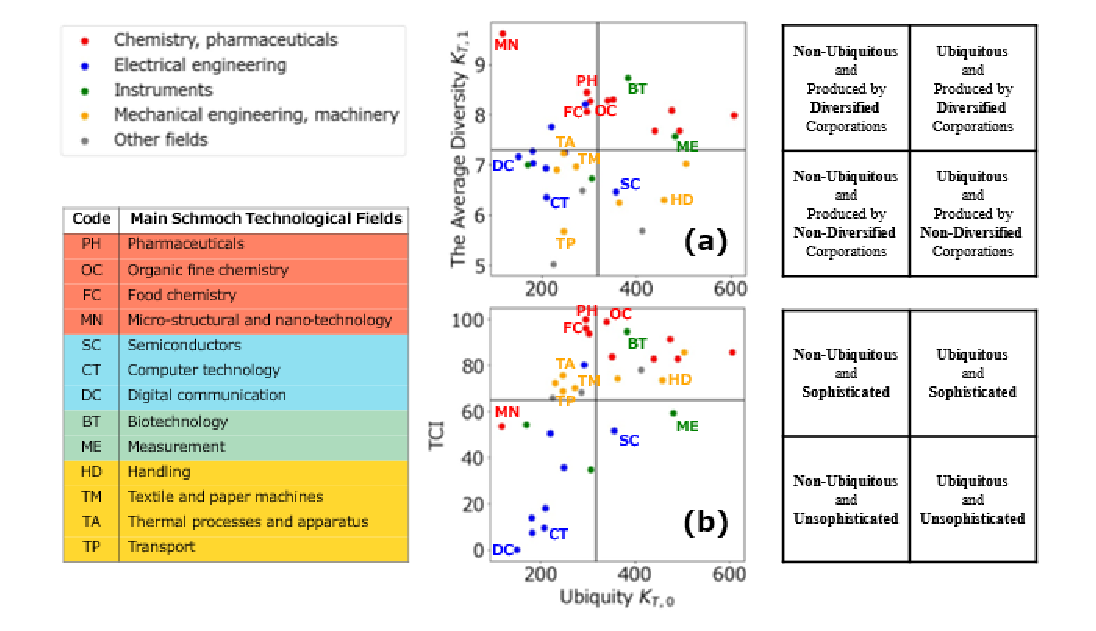
\includegraphics[scale=0.65]{Figs/Fig2.eps}
    \caption{(A) The TCI scores of IPC first Class (N=124) and Schmoch (N=35) for both prefectures and corporations. The scores have been scaled to values ranging from 0 to 100. Each IPC is plotted against the corresponding Schmoch axis, and in cases of multiple correspondences (i.e., ), each pair is plotted individually. (B) The distribution of the absolute differences between TCI of IPC and of Schmoch systems.}
    \label{fig:detailtci}
\end{figure}


\begin{figure}[ht]
    \centering
    \includegraphics[scale=0.35]{Figs/Fig3.eps}
    \caption{Three scatter plots arranged in a single row compare the Corporate TCI in Japan (vertical axis) to the Corporate TCI in Tokyo (left panel), Osaka (middle panel), and Aichi (right panel) on the horizontal axis. Each axis is scaled from 0 to 100, and the black points represent data points for each classification or entity. The red dashed line indicates the diagonal (y = x).}
    \label{fig:prefcompare}
\end{figure}